\documentclass[6pt]{../../shared/AiTex}
\usepackage{csvsimple}

\title{Memoria entrega 2}
\author{A.L.K.}
\date{Febrero 2024}

\begin{document}
%\datos{facultad}{universidad}{grado}{asignatura}{subtitulo}{autor}{curso}
\datos{Informática}{Universidad Complutense de Madrid}{Ingeniería informática}{Aprendizaje Automatico y Big Data}{Entrega 2: regresión lineal de multivariable}{Alejandro Barrachina Argudo}{2023-2024}
% \portadaApuntes
% \pagestyle{empty}
% \tableofcontents
% \pagestyle{empty}
\justify

\begin{center}

    {\huge \textbf{\underline{\subtitulo}}} \\
    { \lesson - \autor}

\end{center}


\section*{Introducción}

En este documento se explicará el código del entregable 2 y el proceso de la regresión lineal en variables múltiples.

Para esta práctica se usarán los siguientes \textit{imports} vistos en la figura \ref{fig:imports}.

\begin{figure}[H]
    \centering
    \lstinputlisting[firstline=1,lastline=6, style=custompython]{../multi_linear_reg.py}
    \caption{Código de las bibliotecas usadas}
    \label{fig:imports}
\end{figure}

\section{Regresión lineal en variables múltiples}

Para esta regresión definimos la función de pendiente como en la figura \ref{fig:fun} como métrica, también se usan las funciones de coste \ref{fig:compute_cost} y de gradiente \ref{fig:compute_gradient} según descritas en los apuntes.

Para hacer el gradiente descendente usamos \ref{fig:gradient_descent} con 1000 iteraciones, 0.01 en $\alpha$ y 0 para iniciar w y b.

Si no hacemos una normalización de los datos, estos procesos darán pesos bastante dispares e incorrectos a los distintos campos de predicción, para ello usamos la función `zscore\_normalize\_features' (figura \ref{fig:normalize}) que normaliza los datos de la entrada dados.

\begin{figure}[H]
    \centering
    \lstinputlisting[firstline=9,lastline=21, style=custompython]{../multi_linear_reg.py}
    \caption{Código de la función `fun'}
    \label{fig:fun}
\end{figure}

\begin{figure}[H]
    \centering
    \lstinputlisting[firstline=43,lastline=60, style=custompython]{../multi_linear_reg.py}
    \caption{Código de la función `compute\_cost'}
    \label{fig:compute_cost}
\end{figure}

\begin{figure}[H]
    \centering
    \lstinputlisting[firstline=63,lastline=83, style=custompython]{../multi_linear_reg.py}
    \caption{Código de la función `compute\_gradient'}
    \label{fig:compute_gradient}
\end{figure}

\begin{figure}[H]
    \centering
    \lstinputlisting[firstline=86,lastline=121, style=custompython]{../multi_linear_reg.py}
    \caption{Código de la función `gradient\_descent'}
    \label{fig:gradient_descent}
\end{figure}

\begin{figure}
    \centering
    \lstinputlisting[firstline=24,lastline=40, style=custompython]{../multi_linear_reg.py}
    \caption{Código de la función `zscore\_normalize\_features'}
    \label{fig:normalize}
\end{figure}

\section{Gráficas}

La primera gráfica a generar es la que nos muestra los datos brutos (figura \ref{fig:data}), viendo así como se relaciona cada característica con el precio de una vivienda, para ello usamos la función `visualize\_data' \ref{fig:visualize_data}. Tras el entrenamiento del modelo podemos ver en la figura \ref{fig:data_train} la predicción de precios y los datos dados, este gráfico lo generamos con la función `visualize\_data\_train' (figura \ref{fig:visualize_data_train}).

También podemos observar la evolución de la función de coste en la figura \ref{fig:cost} con la función `visualize\_J\_history' (figura \ref{fig:visualize_J_history}) y las regresiones parciales en la figura \ref{fig:reg_parciales}, producidas por la función `visualize\_partial\_regression' (figura \ref{fig:visualize_partial_reggression}).

\begin{figure}[H]
    \centering
    \lstinputlisting[firstline=124,lastline=138, style=custompython]{../multi_linear_reg.py}
    \caption{Código de la función `visualize\_data'}
    \label{fig:visualize_data}
\end{figure}

\begin{figure}[H]
    \centering
    \lstinputlisting[firstline=141,lastline=156, style=custompython]{../multi_linear_reg.py}
    \caption{Código de la función `visualize\_data\_train'}
    \label{fig:visualize_data_train}
\end{figure}

\begin{figure}[H]
    \centering
    \lstinputlisting[firstline=159,lastline=177, style=custompython]{../multi_linear_reg.py}
    \caption{Código de la función `visualize\_partial\_regression'}
    \label{fig:visualize_partial_reggression}
\end{figure}

\begin{figure}[H]
    \centering
    \lstinputlisting[firstline=180,lastline=193, style=custompython]{../multi_linear_reg.py}
    \caption{Código de la función `visualize\_J\_history'}
    \label{fig:visualize_J_history}
\end{figure}

\begin{figure}[H]
    \centering
    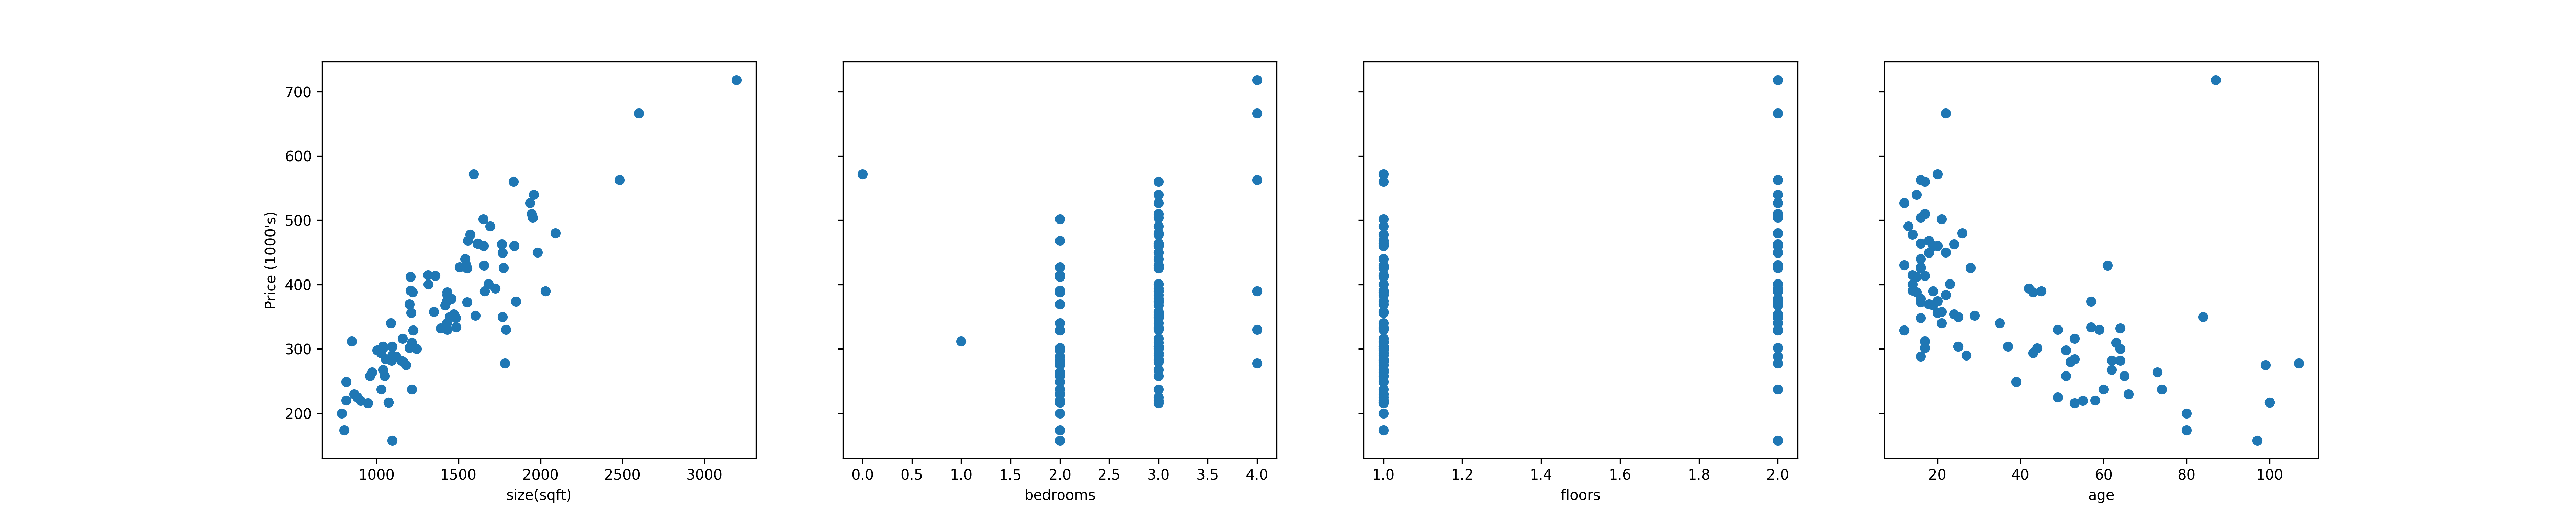
\includegraphics[width=\textwidth]{./images/visualizacion_inicial.png}
    \caption{Visualización de los datos iniciales}
    \label{fig:data}
\end{figure}

\begin{figure}[H]
    \centering
    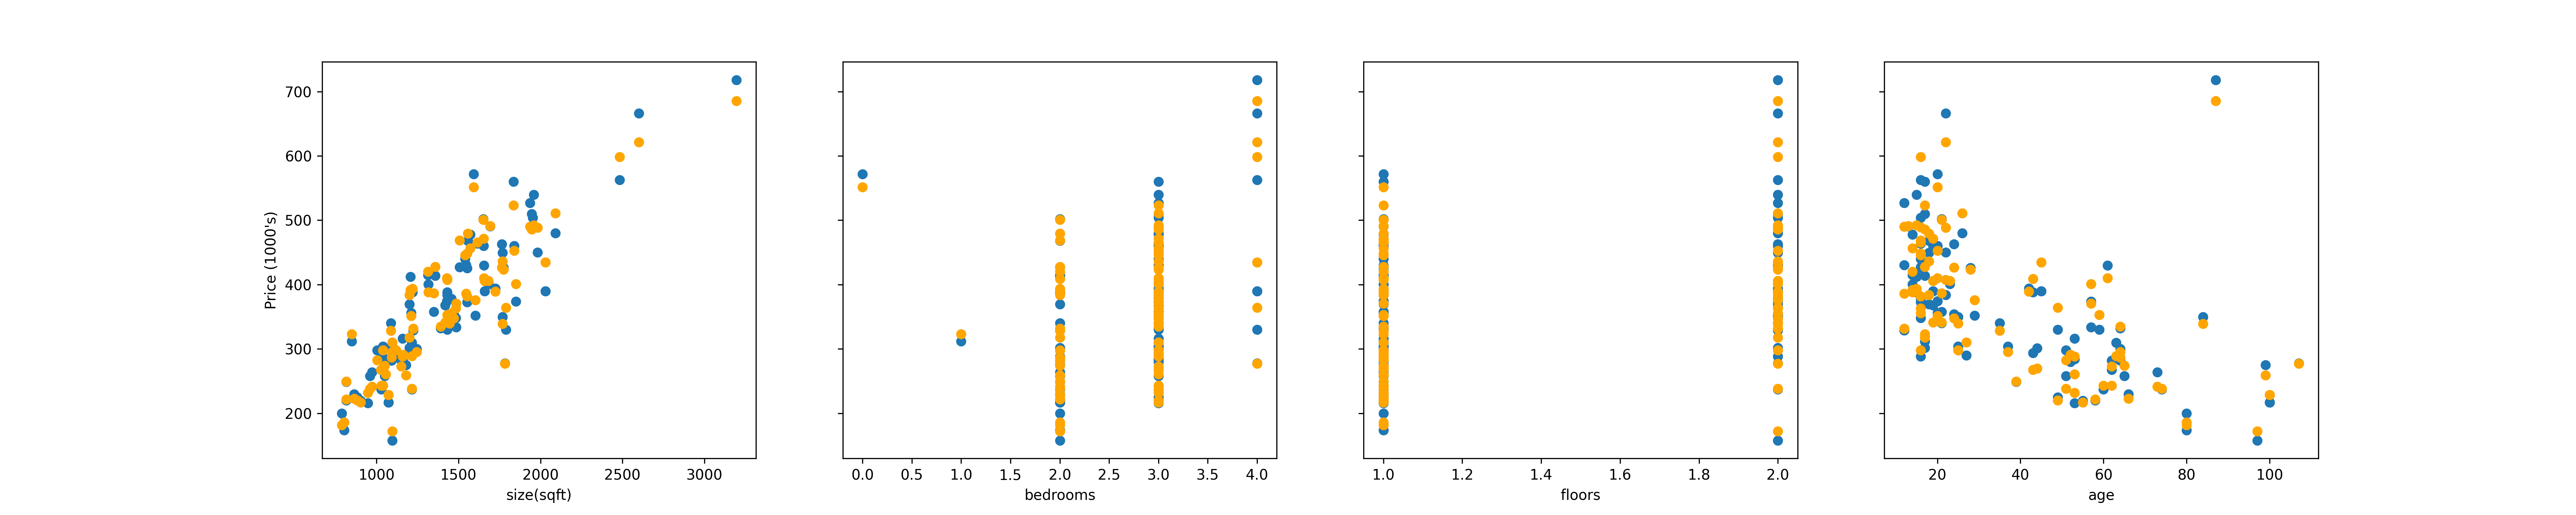
\includegraphics[width=\textwidth]{./images/predicted_data.png}
    \caption{Visualización de los datos predichos}
    \label{fig:data_train}
\end{figure}

\begin{figure}[H]
    \centering
    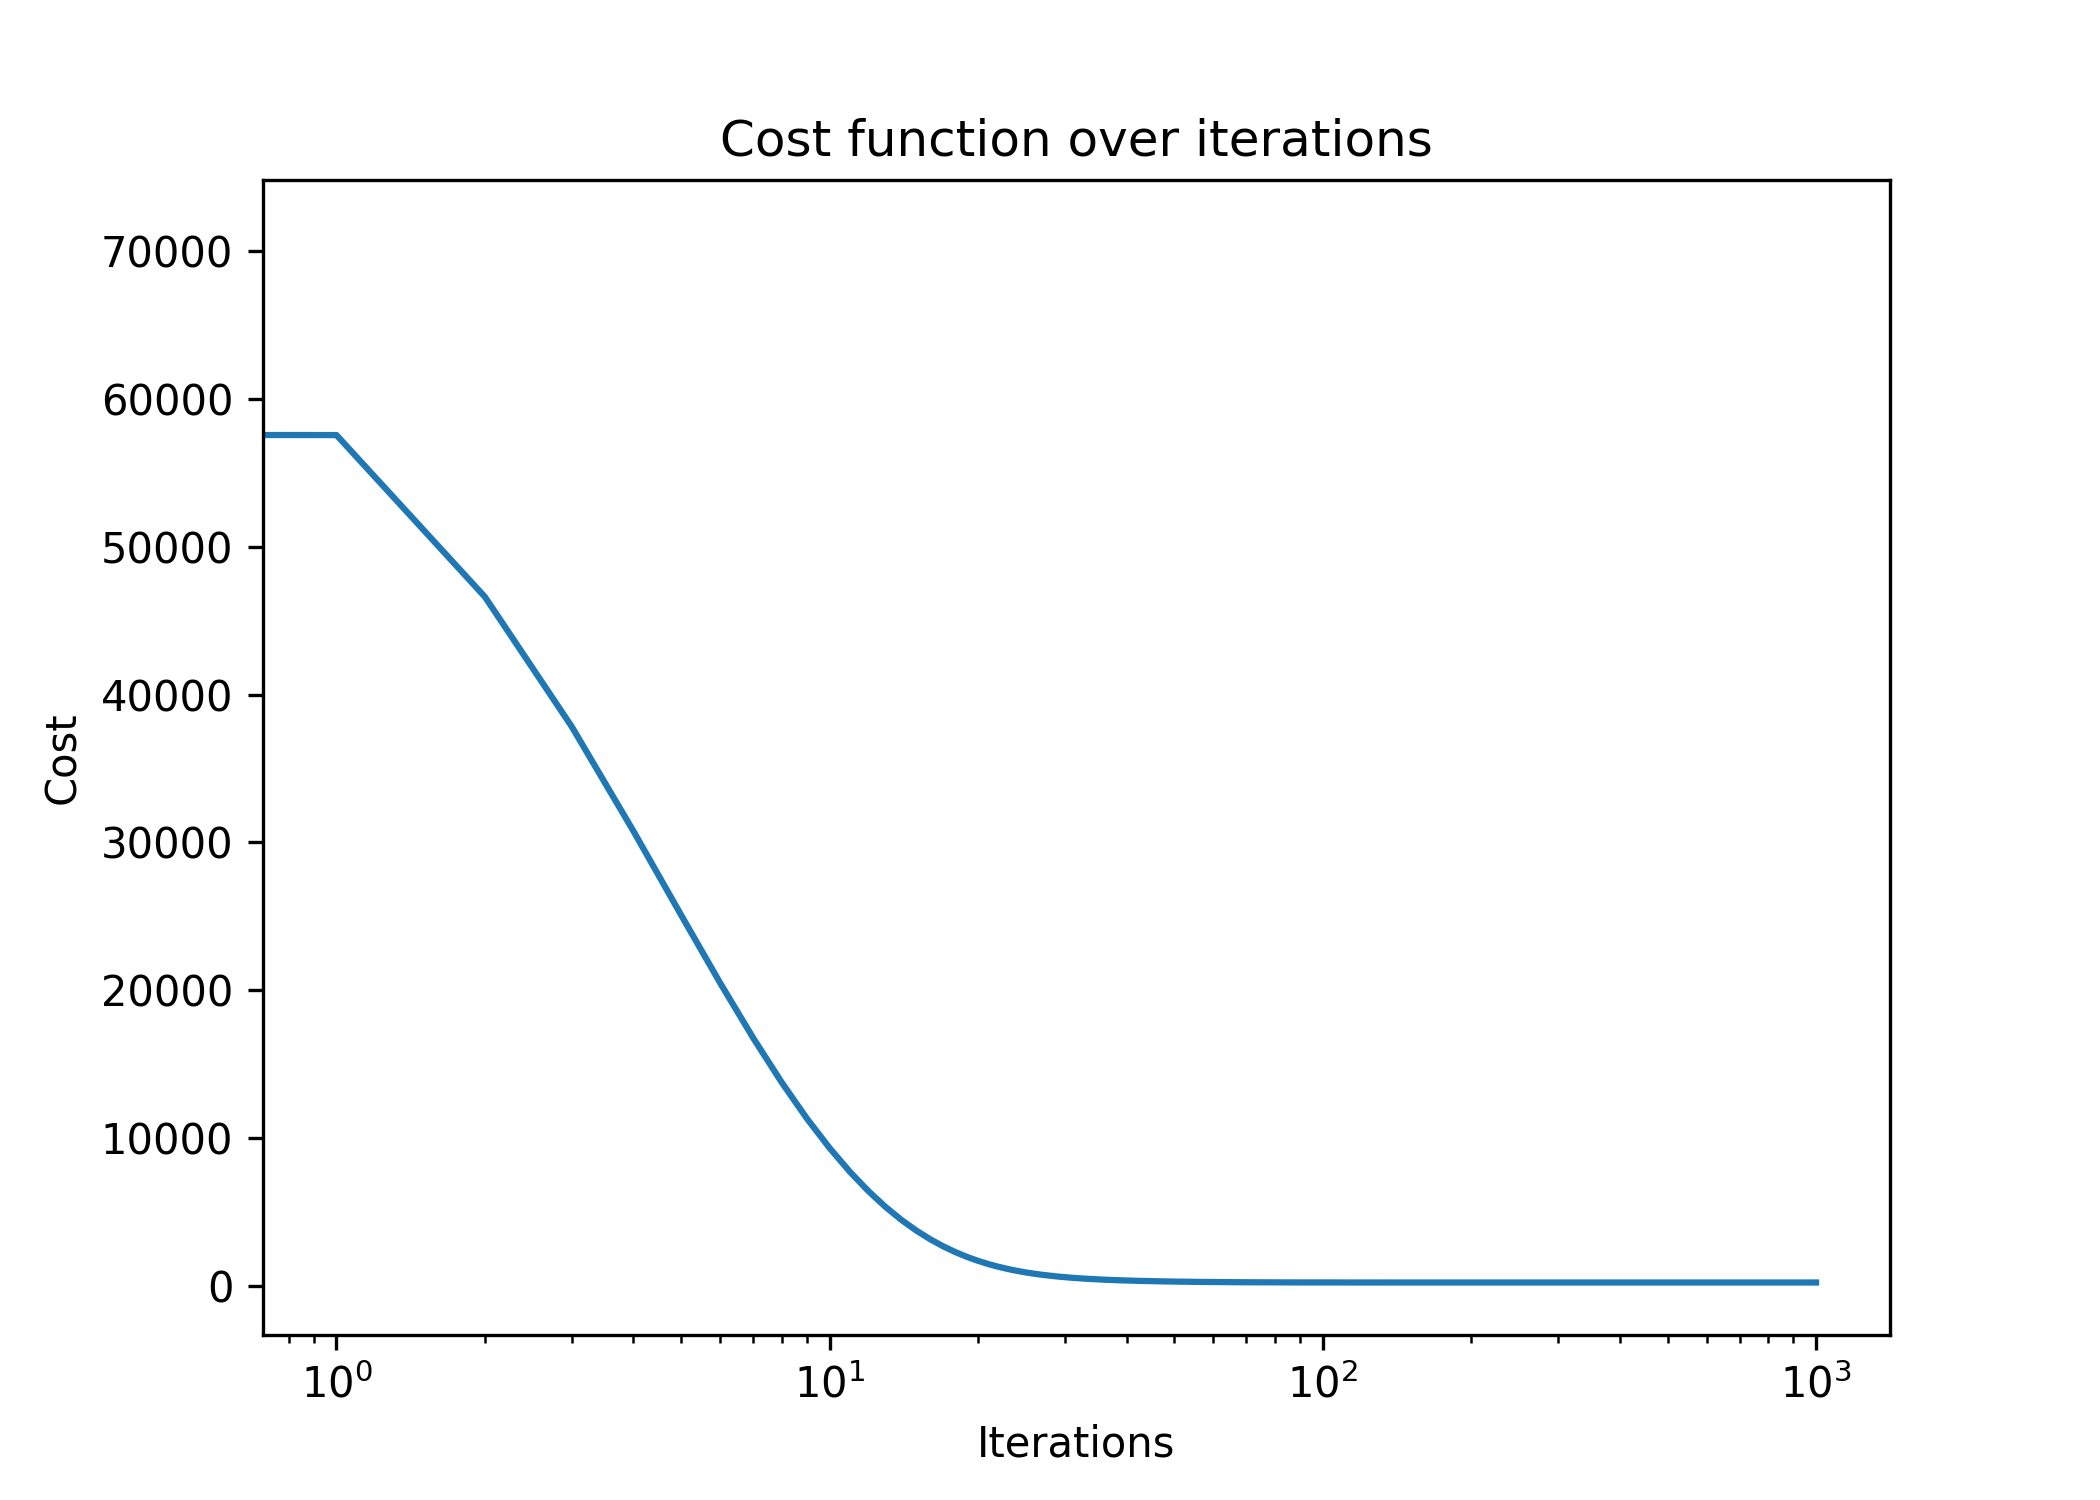
\includegraphics[width=0.6\textwidth]{./images/cost_function.png}
    \caption{Evolución de la función de coste}
    \label{fig:cost}
\end{figure}

\begin{figure}[H]
    \centering
    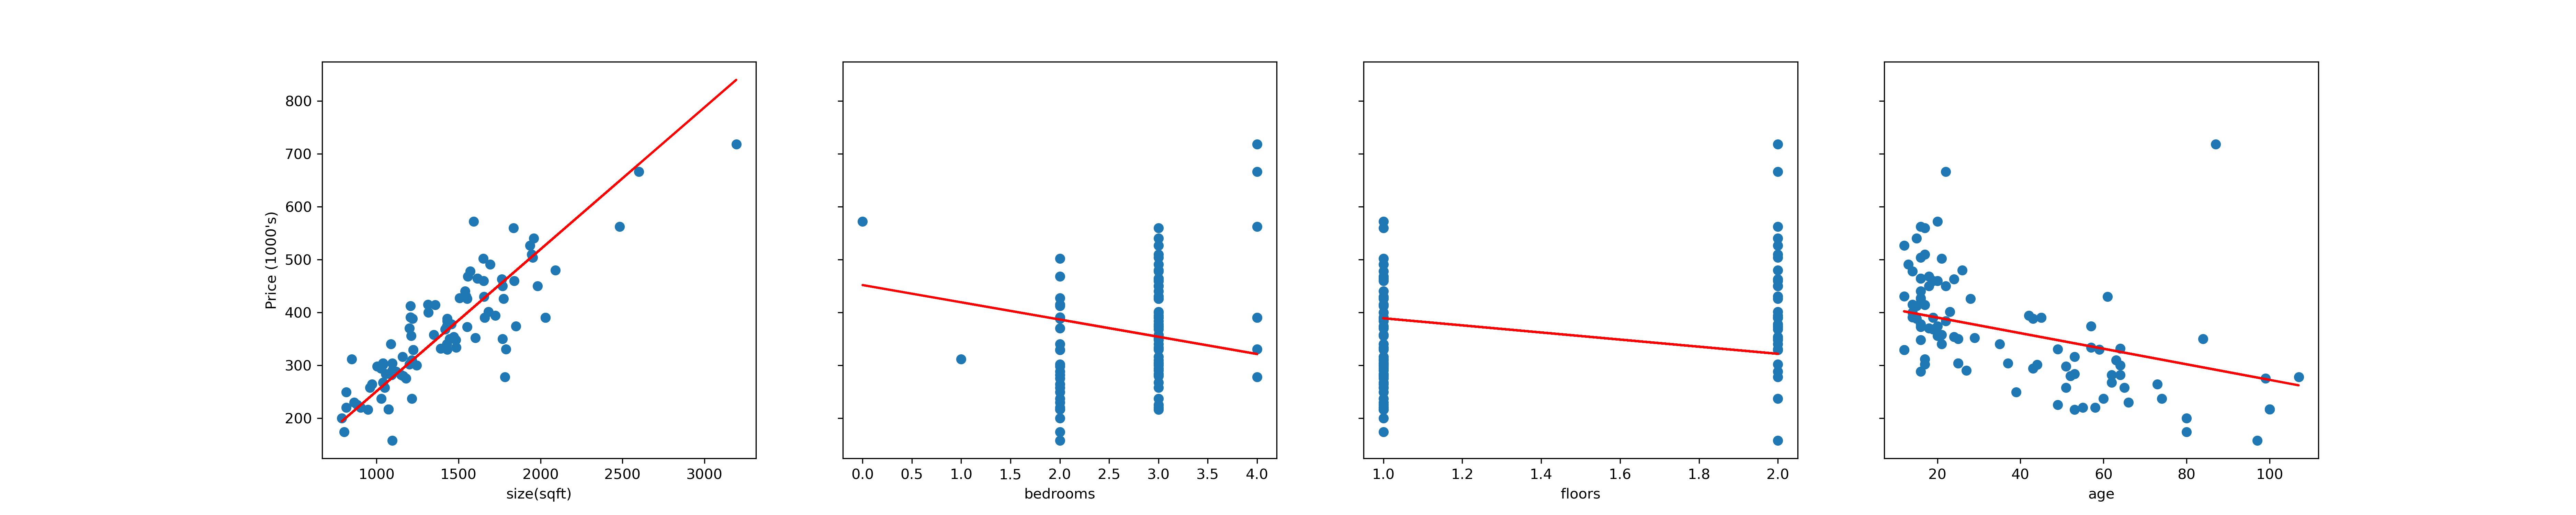
\includegraphics[width=\textwidth]{./images/partial_regression.png}
    \caption{Regresiones parciales}
    \label{fig:reg_parciales}
\end{figure}

\section{conclusiones}

Este modelo al tener más variables produce mejores predicciones que el modelo de la práctica anterior, ya que el anterior solo tenía en cuenta una variable arbitraria.

Para tener más presentes los resultados, usamos la función `write\_results' (figura \ref{fig:write_results}) que nos escribe en un archivo csv los resultados de la predicción. Los resultados finales son:

\begin{table}[H]
    \centering
    \csvreader[tabular=|c|r|,
        table head=\hline \textbf{Iteraciones} & \textbf{J(w,b)} \\ \hline,
        late after line=\\ \hline]
    {./recursos/j_history_simplificado.csv}{1=\casos,2=\iterativo}
    {\casos & \iterativo}
    \caption{Evolución de J(w,b)}
    \label{table:j_history}
\end{table}

\begin{table}[H]
    \centering
    \csvreader[tabular=|c|c|c|c|,
        table head=\hline \textbf{size(sqft)} & \textbf{Bedrooms} & \textbf{floors} & \textbf{age} \\ \hline,
        late after line=\\ \hline]
    {./recursos/mean.csv}{1=\size,2=\bedrooms,3=\floors,4=\age}
    {\size & \bedrooms & \floors & \age}
    \caption{Medias de cada atributo para la normalización}
    \label{table:medias}
\end{table}
\begin{table}[H]
    \centering
    \csvreader[tabular=|c|c|c|c|,
        table head=\hline \textbf{size(sqft)} & \textbf{Bedrooms} & \textbf{floors} & \textbf{age} \\ \hline,
        late after line=\\ \hline]
    {./recursos/sigma.csv}{1=\size,2=\bedrooms,3=\floors,4=\age}
    {\size & \bedrooms & \floors & \age}
    \caption{Desviación estándar de cada atributo para la normalización}
    \label{table:sigma}
\end{table}

\begin{table}[H]
    \centering
    \csvreader[tabular=|c|c|c|c|c|,
        table head=\hline \textbf{W. size(sqft)} & \textbf{W. Bedrooms} & \textbf{W. floors} & \textbf{W. age} & \textbf{b}\\ \hline,
        late after line=\\ \hline]
    {./recursos/wb.csv}{1=\size,2=\bedrooms,3=\floors,4=\age, 5=\b}
    {\size & \bedrooms & \floors & \age & \b}
    \caption{Pesos y bias finales para el modelo}
    \label{table:wb}
\end{table}

\begin{figure}[H]
    \centering
    \lstinputlisting[firstline=196,lastline=216, style=custompython]{../multi_linear_reg.py}
    \caption{Código de la función `write\_results'}
    \label{fig:write_results}
\end{figure}
\end{document}
